% Uncomment this to make slides with overlays:
%\documentclass[slides]{beamer}

% Uncomment these (but comment the above \documentclass line) to make handouts:
\documentclass[handout]{beamer}

% Uncomment these to have more than one slide per page
\usepackage{pgfpages}
\pgfpagesuselayout{2 on 1}[border shrink=5mm]
\pgfpageslogicalpageoptions{1}{border code=\pgfusepath{stroke}}
\pgfpageslogicalpageoptions{2}{border code=\pgfusepath{stroke}}

\usepackage[]{graphicx, color, hyperref}

\mode<presentation>
{
	%\usetheme[secheader]{Boadilla}
	%\usecolortheme[rgb={.835, .102,.169}]{structure}  
	\usetheme[width= 0cm]{Goettingen}
	%\setbeamercovered{transparent}
}
\setbeamertemplate{navigation symbols}{}
\setbeamertemplate{footline}[frame number]

\definecolor{blue2}{rgb}{0.278,0.278,0.729} 
\newcommand{\blue}[1]{\textcolor{blue2}{#1}}
\newcommand{\white}[1]{\textcolor{white}{#1}}
\newcommand{\red}[1]{\textcolor{red}{#1}}
\newcommand{\xbar}{\overline{x}}
\newcommand{\ybar}{\overline{y}}
\newcommand{\phat}{\widehat{p}}
\newcommand{\prob}{\mbox{Pr}}
\newcommand{\E}{\mathbb{E}}
\newcommand{\Var}{\mbox{Var}}
\newcommand{\cp}{\oplus}
\newcommand{\cm}{\circleddash}

\title{Lecture 4: Sampling Methods + Design of Experiments}
\author{Chapter 1.4.2 + 1.5}
\date{}


\begin{document}
%------------------------------------------------------------------------------
\begin{frame}
\titlepage
\end{frame}
%------------------------------------------------------------------------------


%------------------------------------------------------------------------------
\begin{frame}
\frametitle{Goals for Today}

\begin{itemize}
\item Discuss different types of sampling
\item Designing experiments
\item Very important example:  clinical trials
\item Example of my own designed experiment: Fried Chicken Face Off
\end{itemize}

\end{frame}
%------------------------------------------------------------------------------


%------------------------------------------------------------------------------
\begin{frame}
\frametitle{Recall from Lecture 1.3: Population and Samples}

\begin{center}
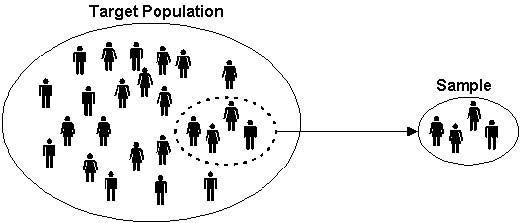
\includegraphics[width=3in]{figure/target-population.jpg} 
\end{center}


\pause If the sample is representative of the desired population then our results are \blue{generalizable}.  

\vskip 0.5cm

\pause How do we take a representative (i.e. unbiased) sample?  You \blue{randomly} sample from the population.

\end{frame}
%------------------------------------------------------------------------------


%------------------------------------------------------------------------------
\begin{frame}
\frametitle{1. Simple Random Sampling}
\begin{center}
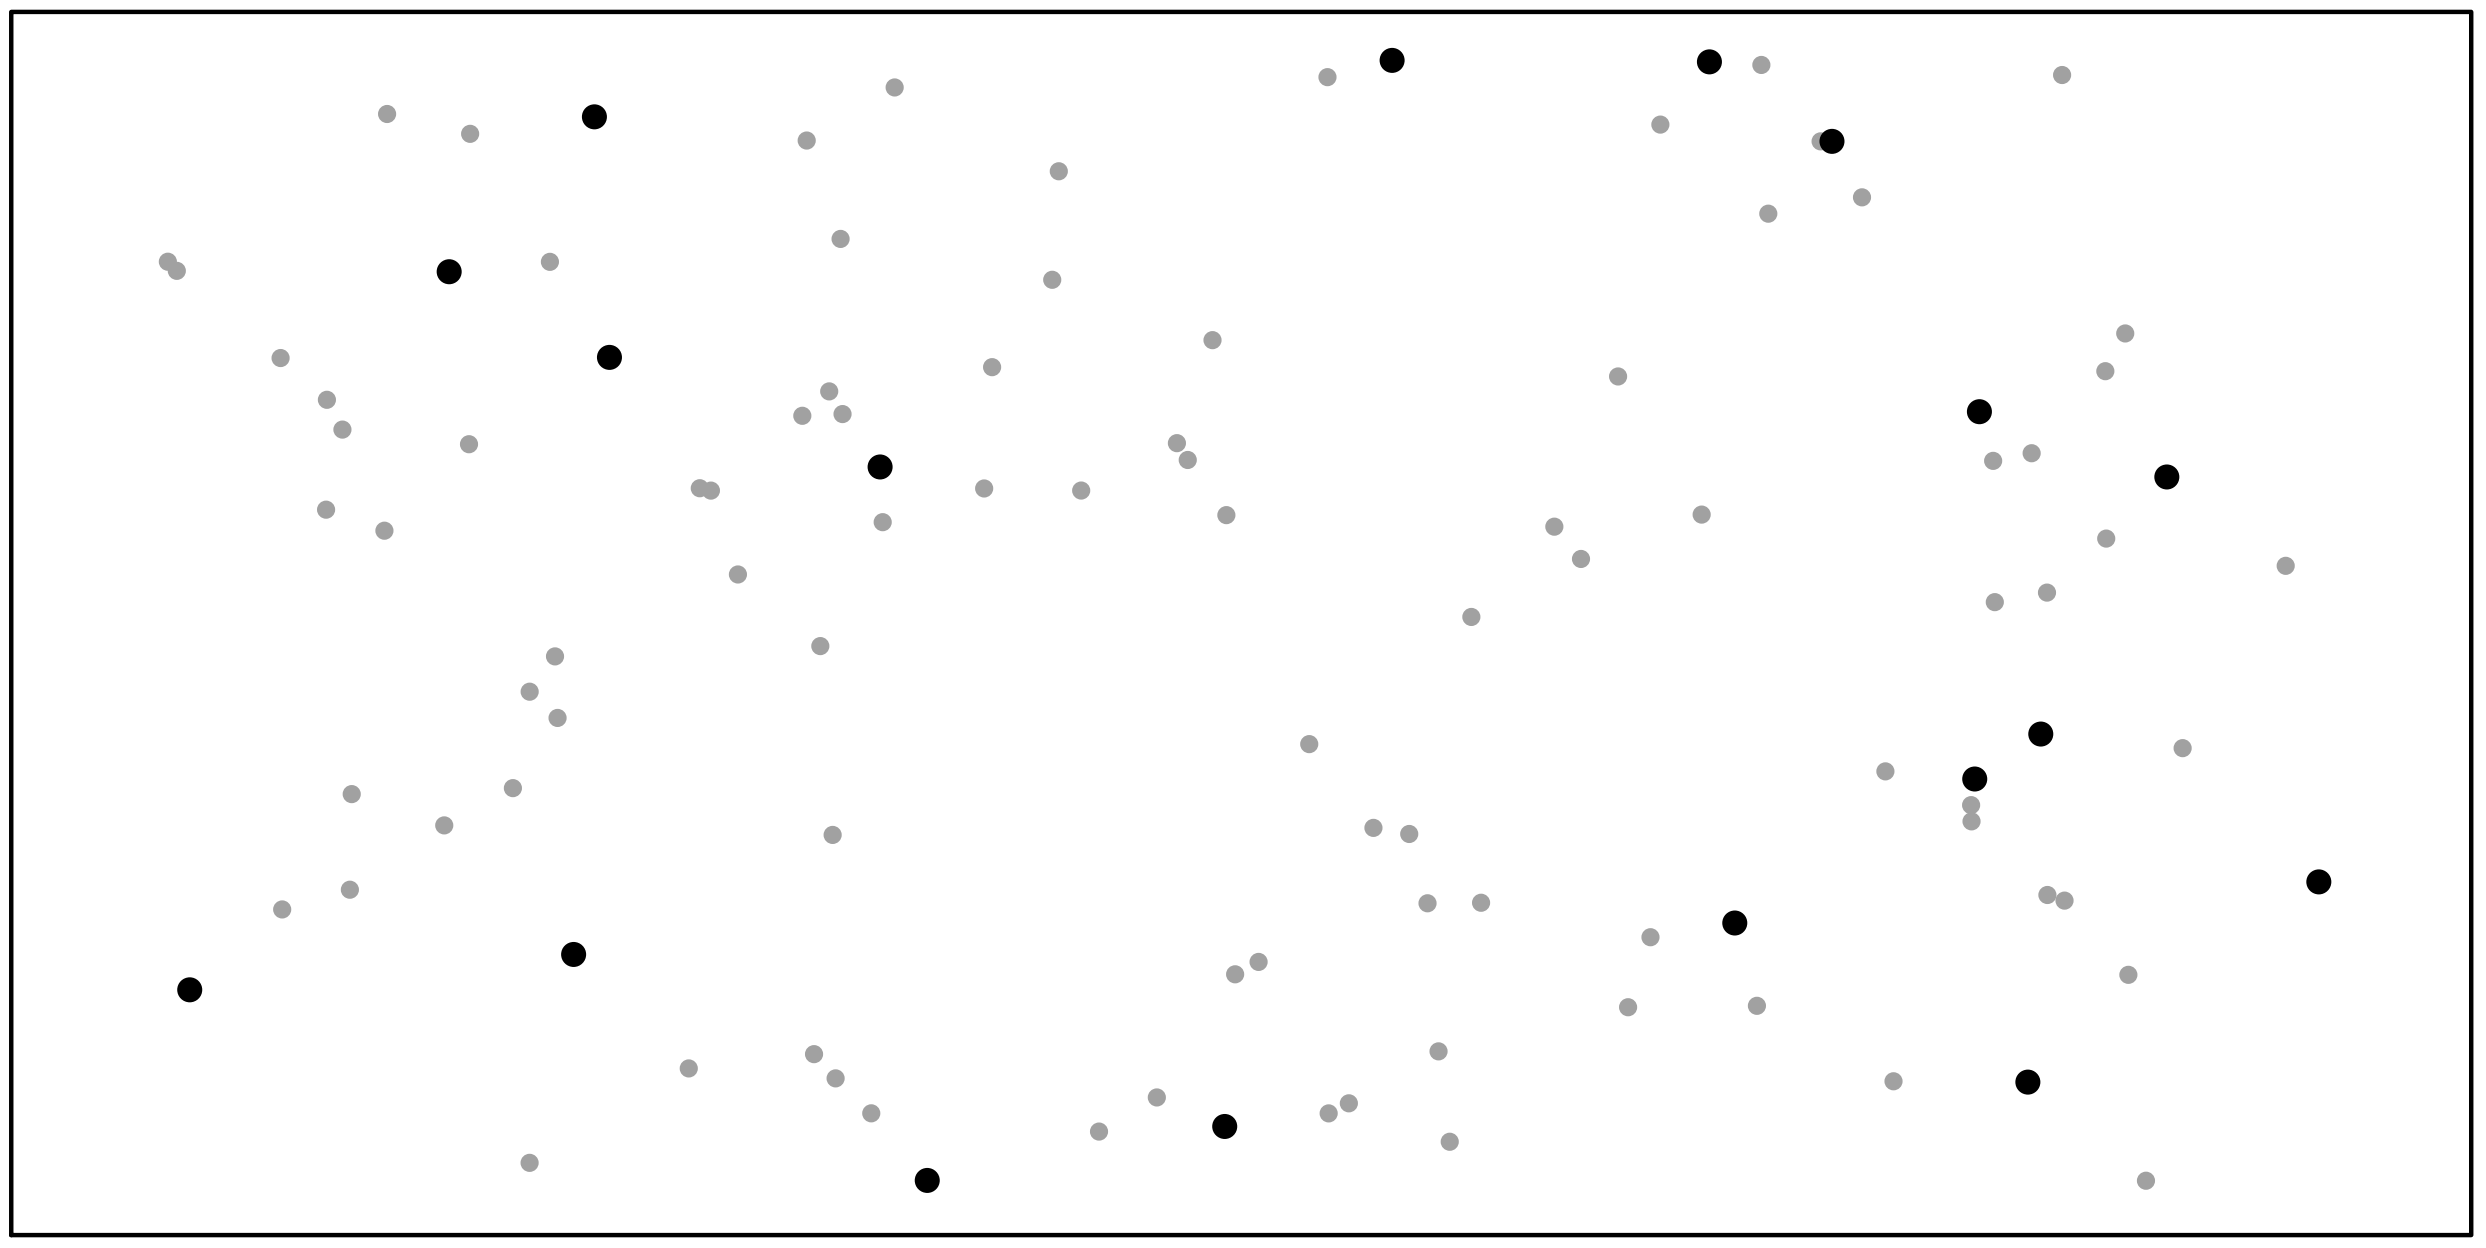
\includegraphics[width=0.75\textwidth]{figure/simple.png}
\end{center}

\blue{Most granular sampling}:  Where every individual in the population has the same probability of being sampled.  \pause Here, all dots are members of the population, and the bolder dots are sampled.  
\end{frame}
%------------------------------------------------------------------------------


%------------------------------------------------------------------------------
\begin{frame}[fragile]
\frametitle{2. Stratified Sampling}

\begin{center}
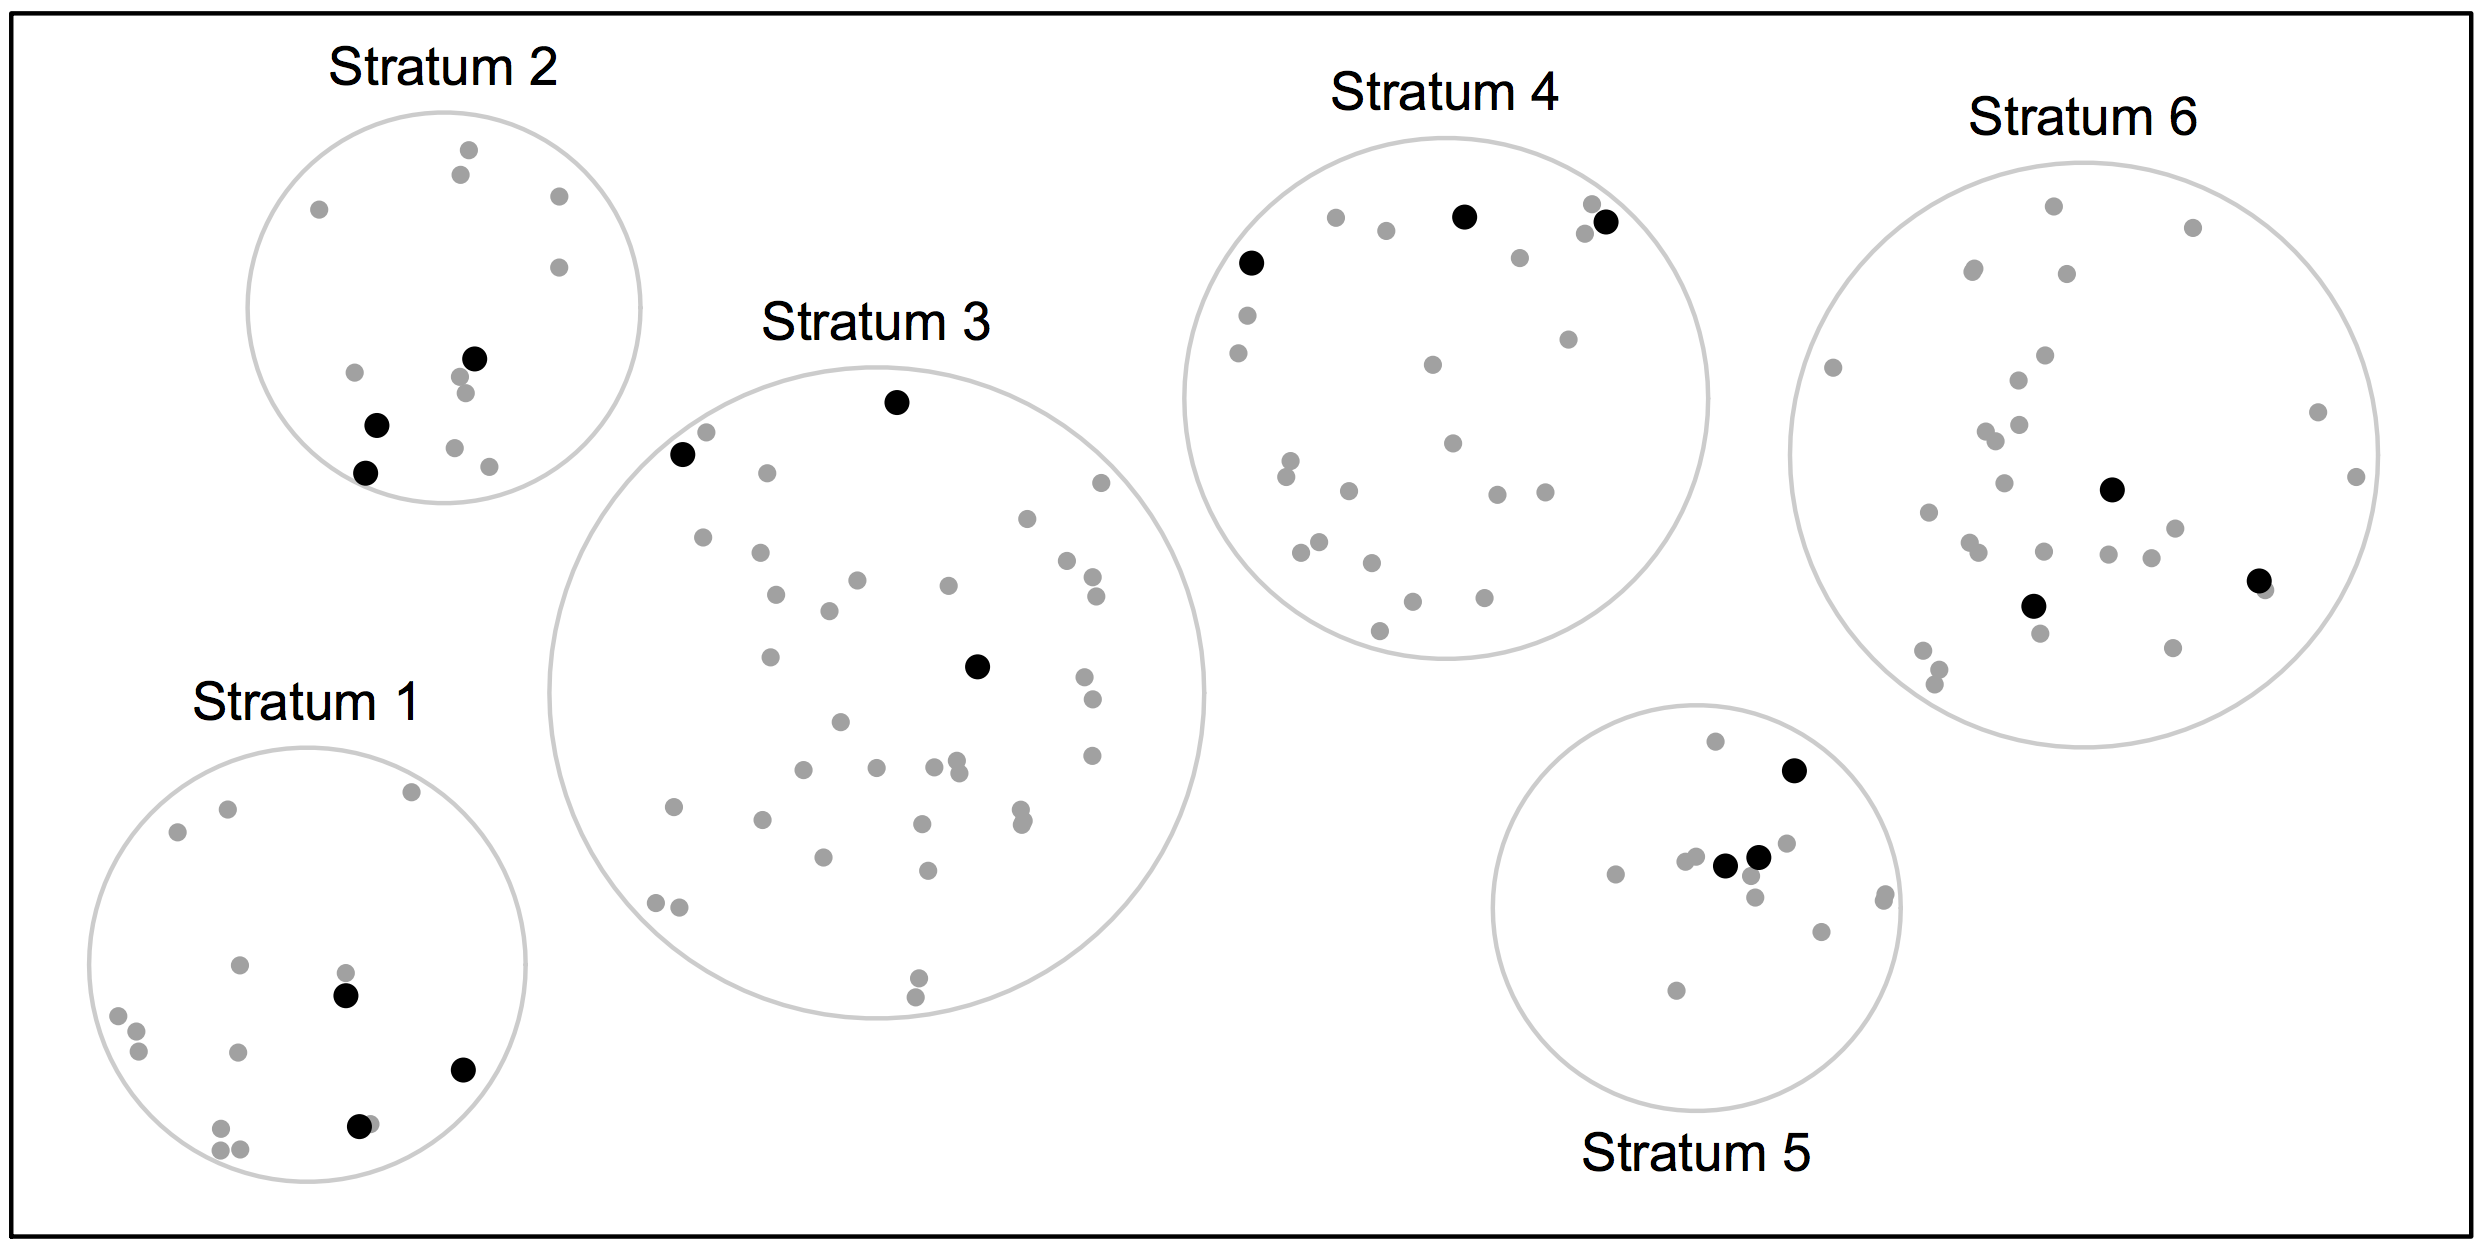
\includegraphics[width=0.75\textwidth]{figure/stratified.png}
\end{center}

\blue{Divide and conquer}:  The population is divided into strata, and we sample from each strata.  \pause For example, each strata could be a census tract in Oregon, and we sample 3 individuals from each strata.  

\end{frame}
%------------------------------------------------------------------------------


%------------------------------------------------------------------------------
\begin{frame}
\frametitle{3. Cluster Sampling}

\begin{center}
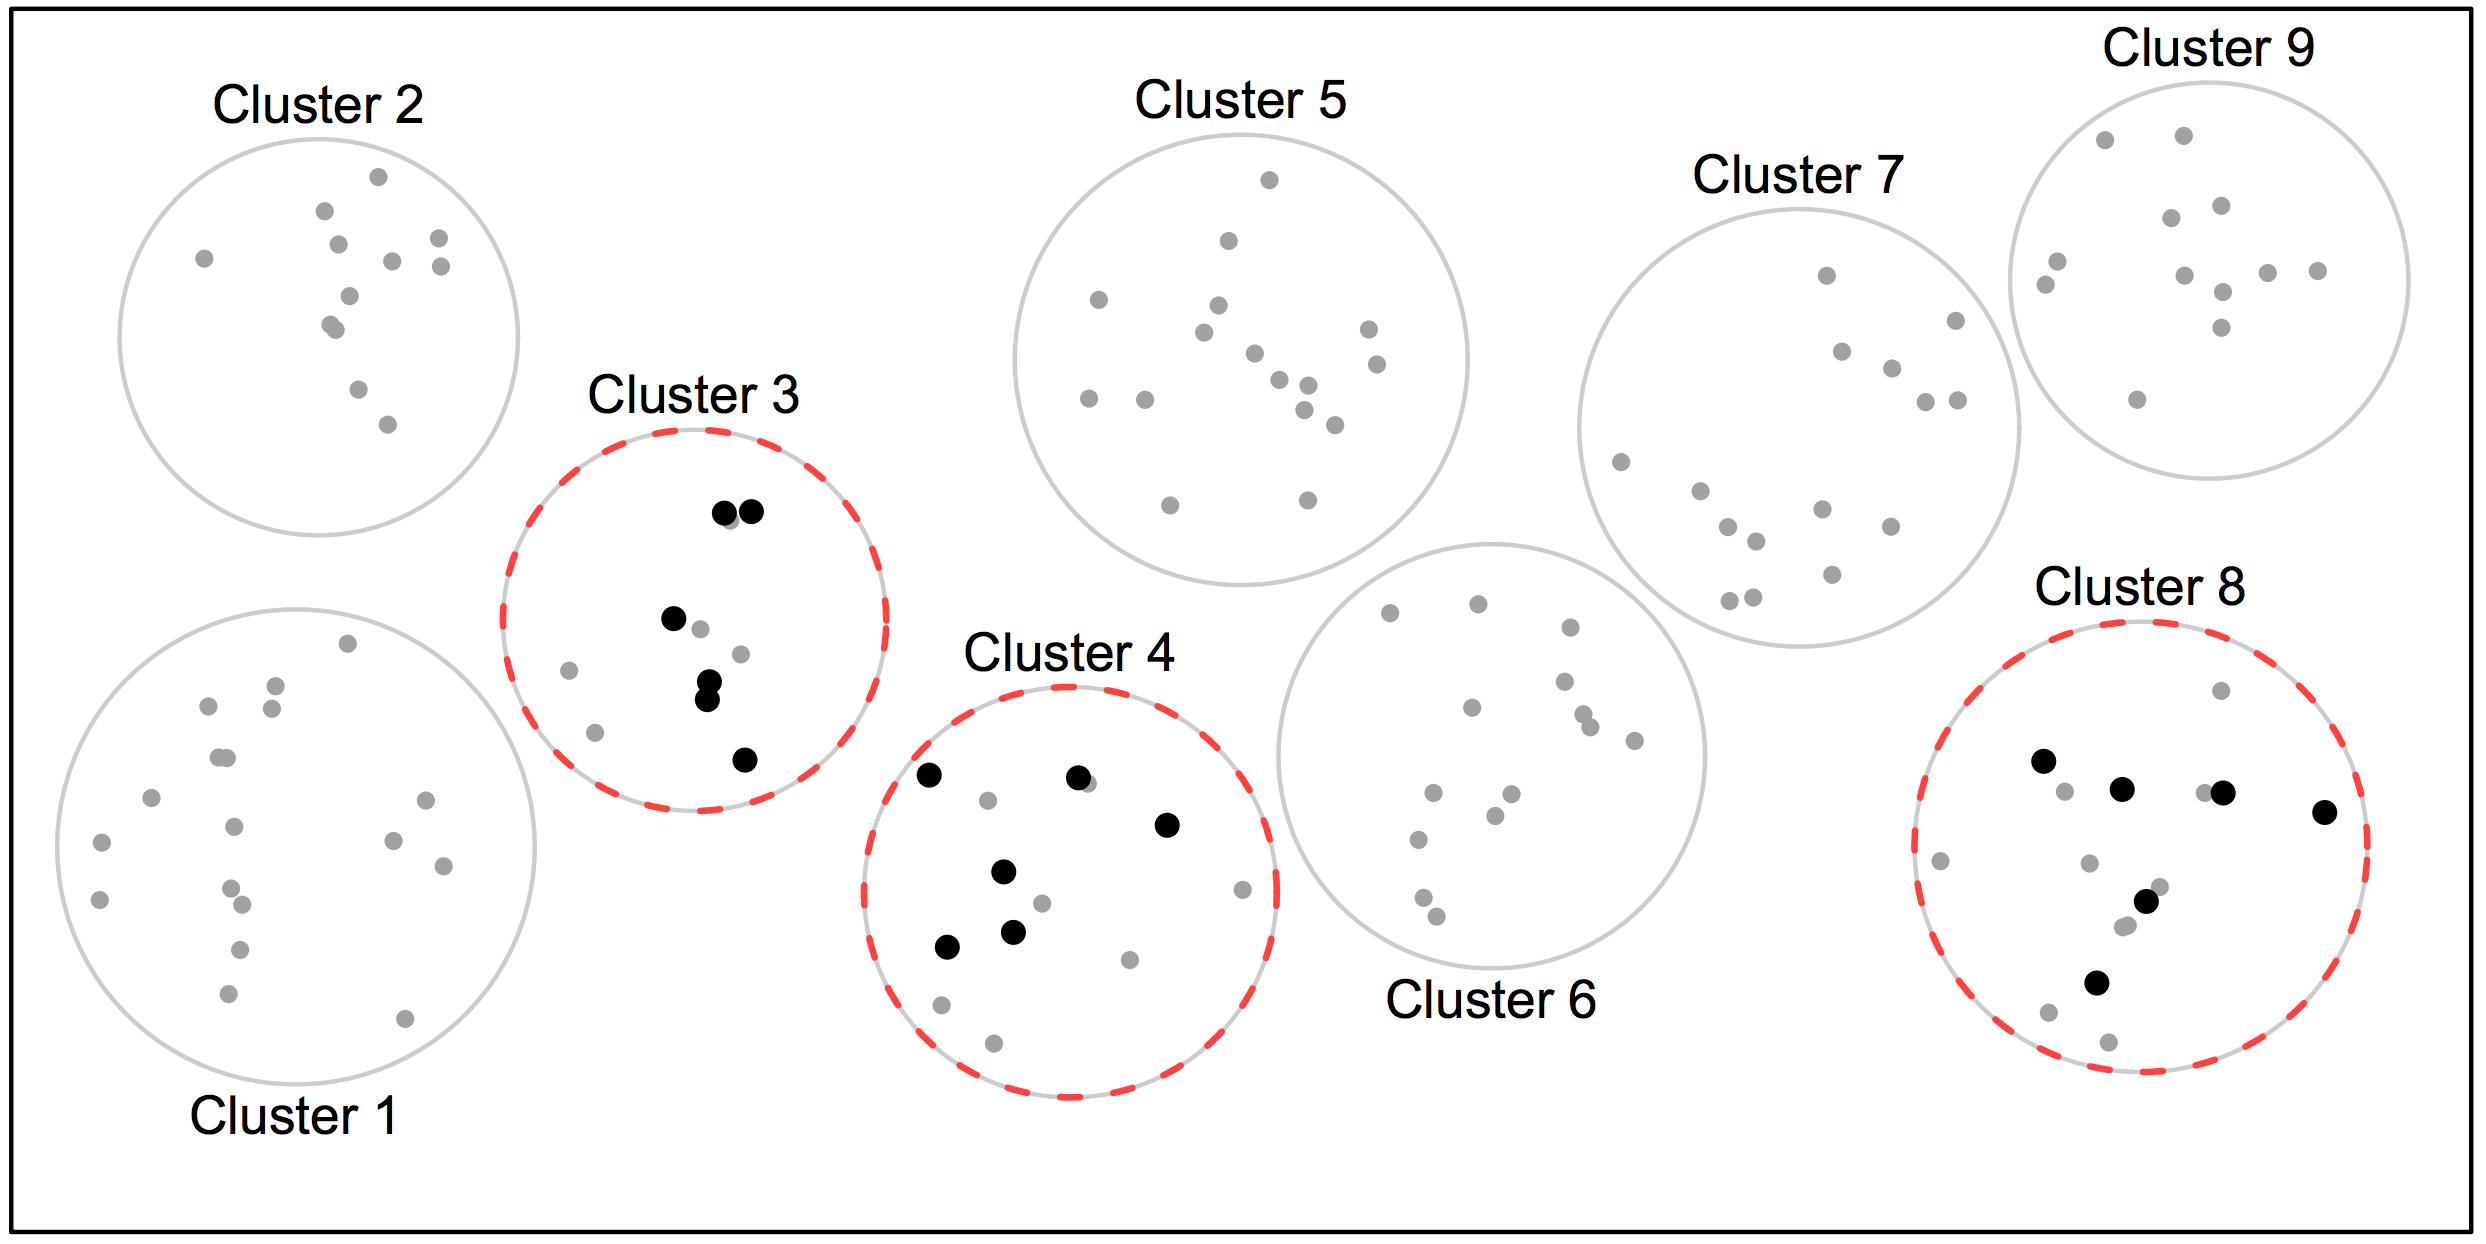
\includegraphics[width=0.75\textwidth]{figure/cluster.png}
\end{center}
\blue{Two stage sampling}:  Very similar to stratified sampling in its process, except that there is no requirement to sample from every cluster.  \pause First the clusters in red were chosen at random, and then we sample from them.
\end{frame}
%------------------------------------------------------------------------------


%------------------------------------------------------------------------------
\begin{frame}
\frametitle{Three Different Types of Sampling}

\begin{enumerate}
\item Simple random sampling: most granular sampling
\item Stratified sampling:  divide and conquer
\item Cluster sampling: two-stage sampling
\end{enumerate}

\vspace{0.5cm}

\pause The mathematics behind the stratified and cluster sampling are more complicated to account for the hierarchies involved.  Ex: for stratified sampling use the Horvitz-Thompson estimator.  

\end{frame}
%------------------------------------------------------------------------------


%------------------------------------------------------------------------------
\begin{frame}
\frametitle{Statistics in Society:  The US Census}

The purpose of the decennial US census is \blue{congressional apportionment}: the 435 seats in the US House of Representatives get distributed to the 50 states in proportion to their population.  \pause After the 2010 census:

\begin{center}
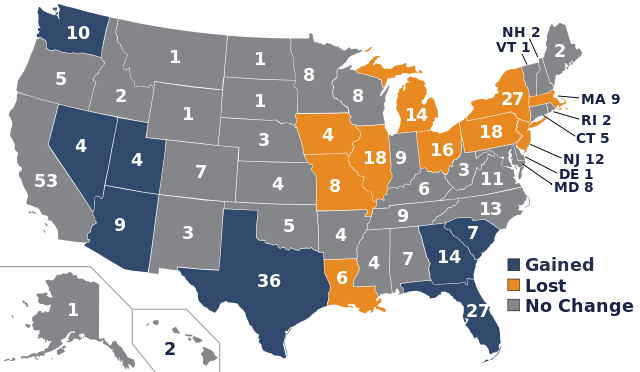
\includegraphics[width=0.8\textwidth]{figure/apportionment.png}
\end{center}



\end{frame}
%------------------------------------------------------------------------------


%------------------------------------------------------------------------------
\begin{frame}
\frametitle{Statistics in Society:  The US Census}

President Bill Clinton's administration planned on using sampling in the 2000 census.  In an article dated in 1996:
\pause \begin{center}
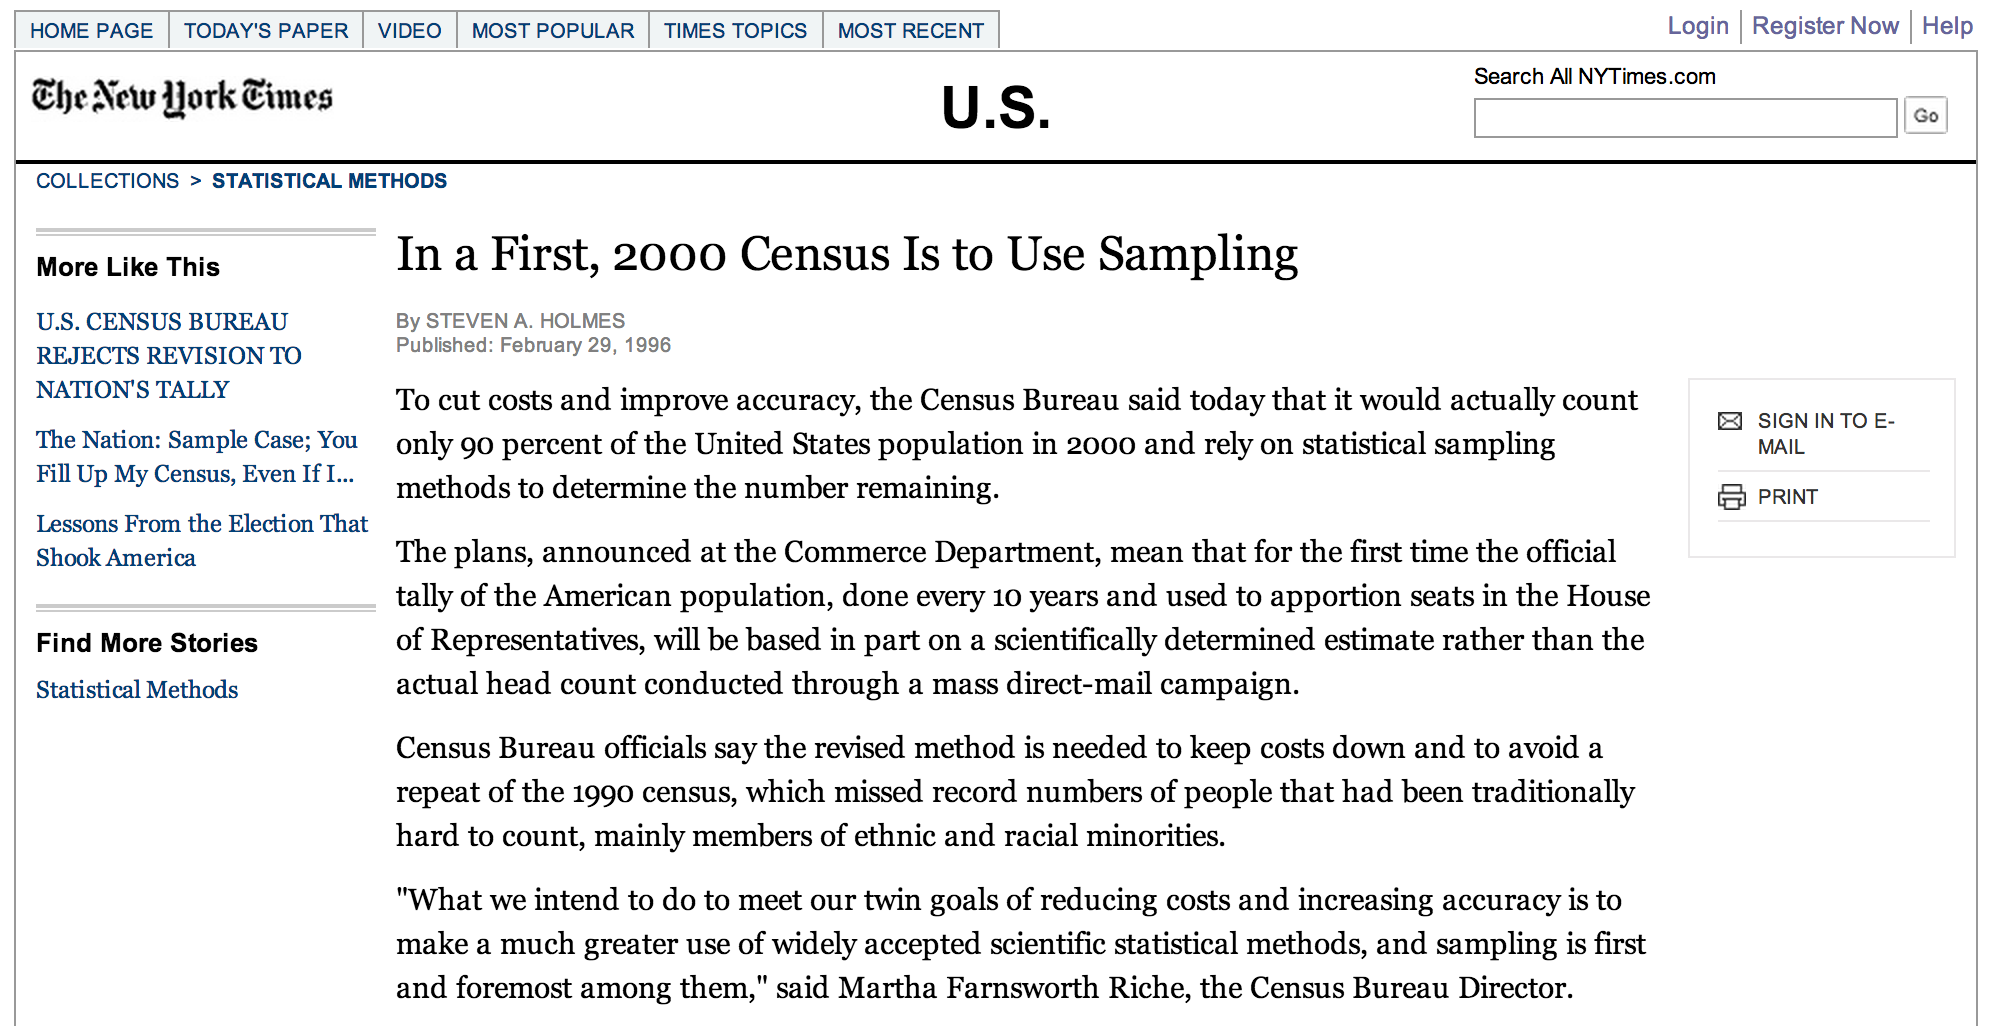
\includegraphics[width=\textwidth]{figure/census_2000.png}
\end{center}

\end{frame}
%------------------------------------------------------------------------------


%------------------------------------------------------------------------------
\begin{frame}
\frametitle{Statistics in Society:  The US Census}

% 
\includegraphics[width=0.5\textwidth]{figure/wethepeople.jpg}

However, Article I, Section 2 of the US Constitution states:  \textit{The \blue{actual Enumeration} shall be made within three Years after the first Meeting of the Congress of the US, and within every subsequent Term of ten Years...}

\vspace{0.25cm}

\pause As such, the Supreme Court ruled 5-4 in 1999 that
\begin{itemize}
\pause\item sampling could not "under any circumstances" be used to reapportion U.S. House seats
\pause\item could be used for other purposes such as redrawing state legislative districts or allocating federal funds to cities and states
\end{itemize}

\end{frame}
%------------------------------------------------------------------------------


%------------------------------------------------------------------------------
\begin{frame}
\frametitle{Statistics in Society:  The Census}
\begin{center}
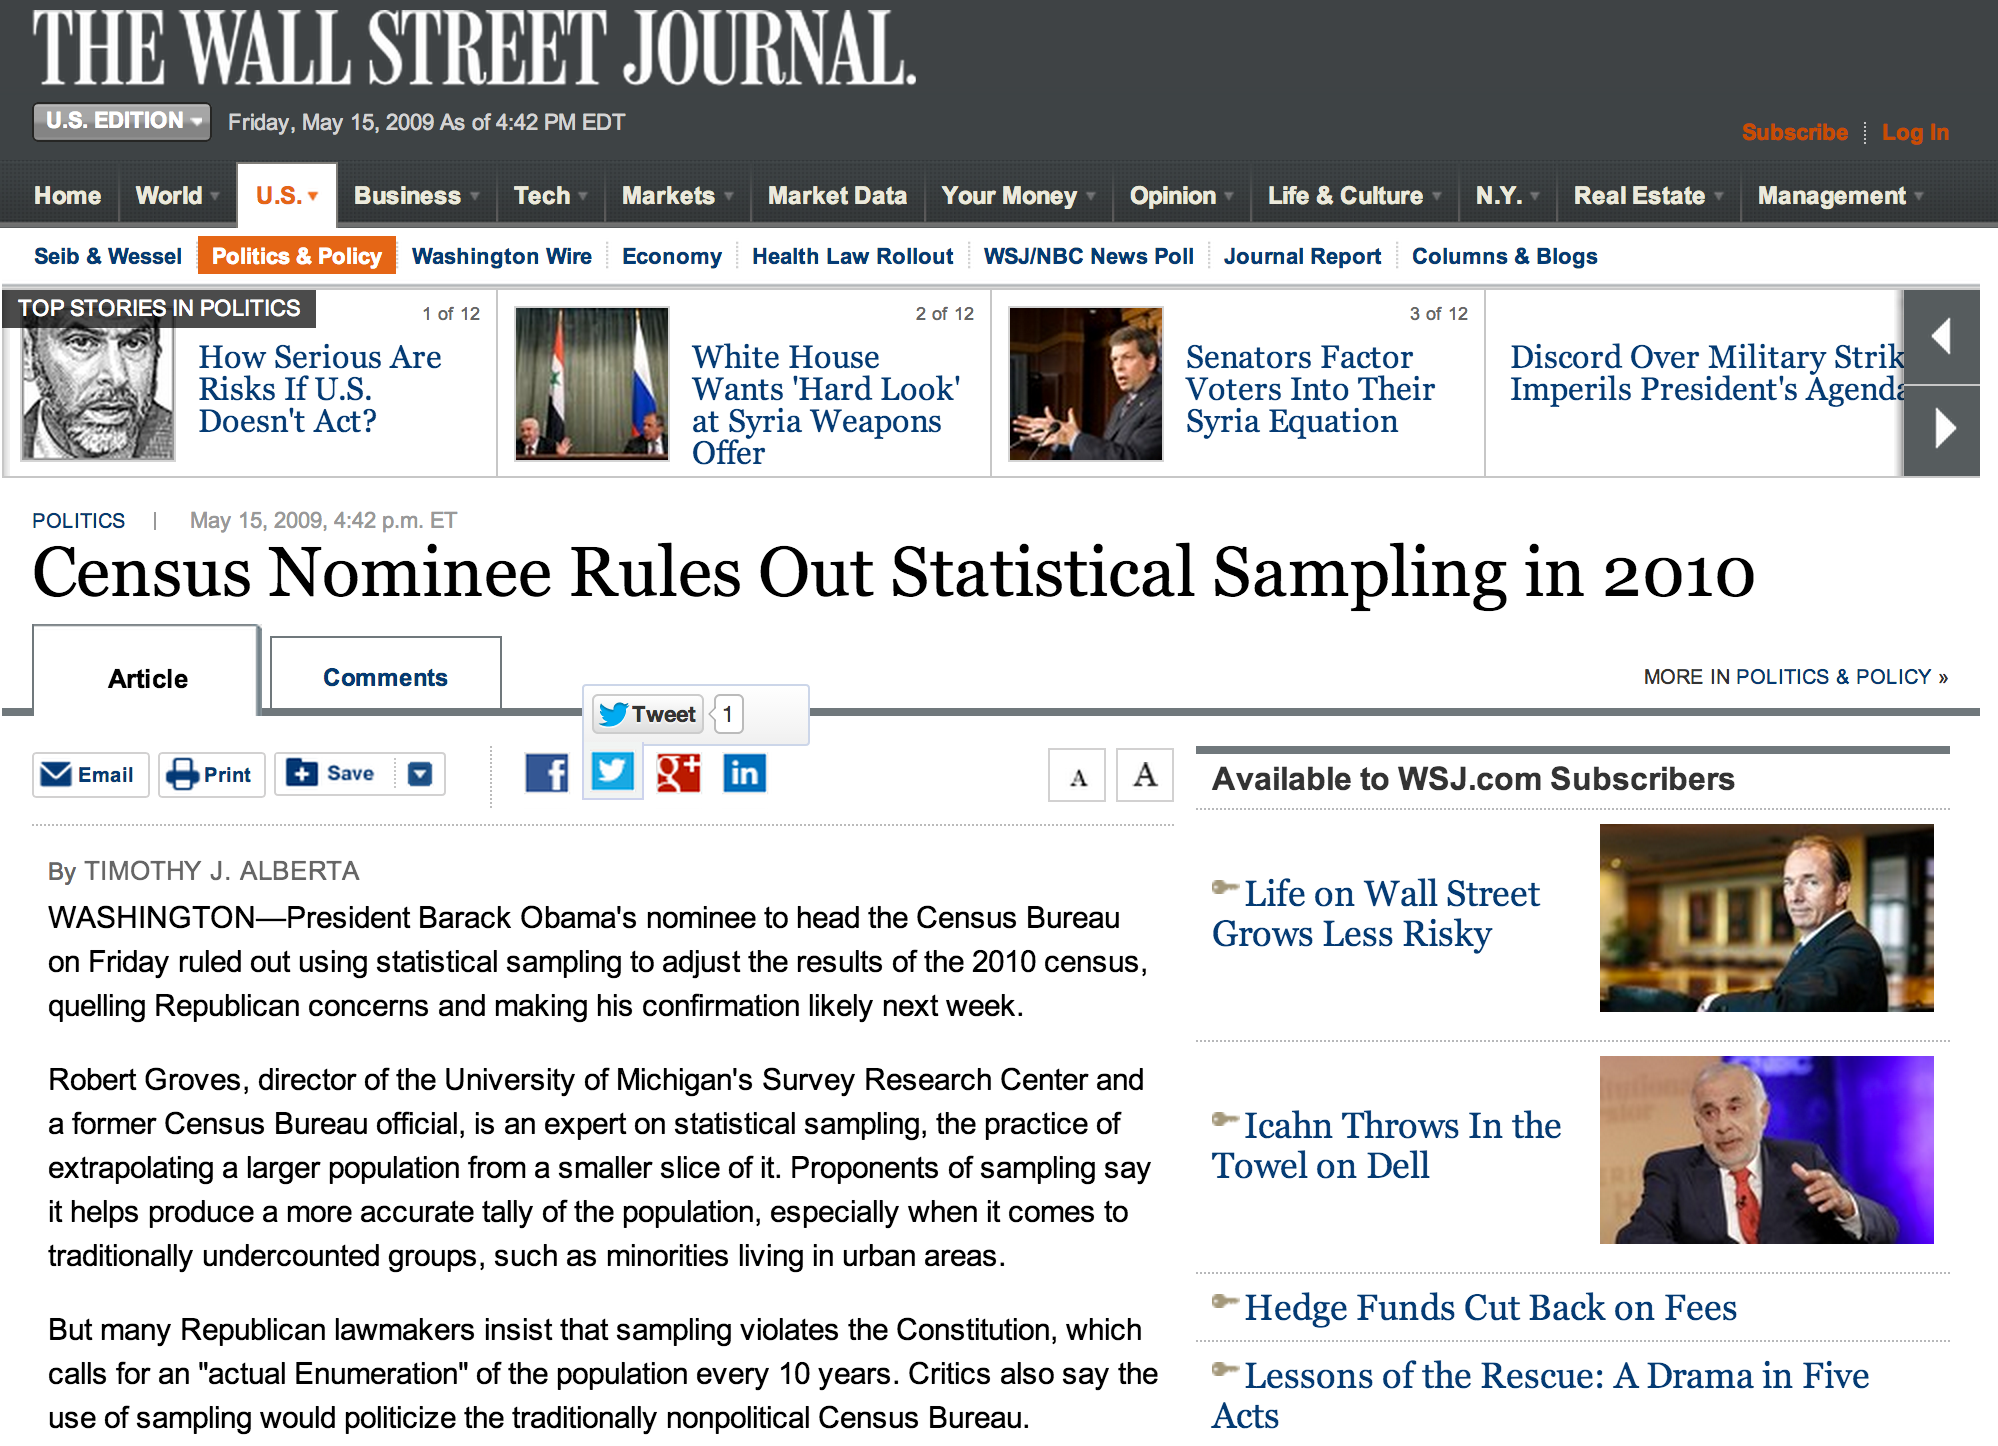
\includegraphics[width=\textwidth]{figure/census_2010.png}
\end{center}

\end{frame}
%------------------------------------------------------------------------------


%------------------------------------------------------------------------------
\begin{frame}
\frametitle{Principles Of Designing Experiments}

Switching gears...

\vspace{0.5cm}

(Wikipedia) In general usage, \blue{design of experiments (DOE) or experimental design} is the design of any information-gathering exercises where variation is present, whether under the full control of the experimenter or not. 

\vspace{0.5cm}

\pause However, in statistics, these terms are usually used for \blue{controlled experiments}: experiments where there is a control and treatment group.

\end{frame}
%------------------------------------------------------------------------------


%------------------------------------------------------------------------------
\begin{frame}
\frametitle{Principles Of Designing Experiments}

%
% Comment this
%
\begin{enumerate}
\pause\item\blue{Controlling}:  We want to control for differences between the two groups.
\pause\item\blue{Randomization}: We randomize individuals into treatment vs control so that any differences in uninteresting variables even out in the long run.  
\pause\item\blue{Replication}:  The more cases we observe, the more ``precise'' the results.
\pause\item\blue{Blocking}:  Researchers sometimes know or suspect that variables, other than the treatment, influence the response. In this case, they may first group individuals based on this variable into blocks and then randomize cases within each block.  
\end{enumerate}

\end{frame}
%------------------------------------------------------------------------------


%------------------------------------------------------------------------------
\begin{frame}
\frametitle{Clinical Trials}

To evaluate the efficacy of a drug, they must be subject to a \blue{clinical trial}.  \pause The gold standard for a clinical trial is \blue{randomized controlled trial}.  i.e. randomized control and treatment groups.  

\vspace{5cm}

%
% Comment this
%
\begin{itemize}
\pause\item \blue{Blinded study}: When researchers do not inform patients which group, or arm, they are in
\pause\item \blue{Double blinded study}:  When the person administering the treatment/control themselves do not know which group the patient is in.
\pause\item \blue{Placebo}: Fake treatment.  Sometimes the \blue{thought} alone of having a treatment is enough to influence behavior/results.  
\pause\item \blue{Phases}. In particular, \blue{pilot studies}.
\end{itemize}

\end{frame}
%------------------------------------------------------------------------------


%------------------------------------------------------------------------------
\begin{frame}
\frametitle{Example of Mine: Ezell's Famous Chicken}
In Seattle's Central District lies
\begin{center}
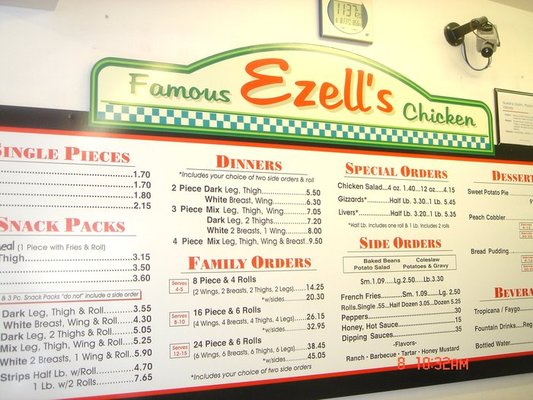
\includegraphics[height=4cm]{figure/ezells.jpg}
\end{center}

\pause From Wikipedia: Oprah Winfrey called it her favorite fried chicken. There are a number of photos of her on the wall of the original restaurant proclaiming her love of the chicken. It is also said she has the chicken flown to her in Chicago when she has a craving.

\end{frame}
%------------------------------------------------------------------------------


%------------------------------------------------------------------------------
\begin{frame}
\frametitle{Example of Mine: Ezell's Famous Chicken}
One day I was raving about Ezell's Chicken.  My friend Nick accused me of being another person ``buying into the hype''; that if people were subjected to a blinded taste test, Ezell's would fare no better than KFC.  So...

\vspace{0.25cm}

\pause\begin{center}
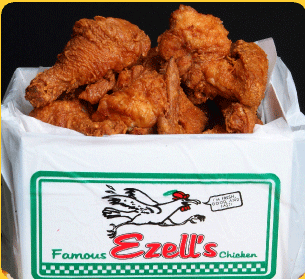
\includegraphics[height=3cm]{figure/ezells2.png} \hspace{0.5cm} vs \hspace{0.5cm} 

\includegraphics[height=3cm]{figure/KFC.png}
\end{center}

\vspace{0.25cm}

We set up a ``Fried Chicken Face Off'' where we would have individuals try both kinds of chicken and rate which one they liked more.  


\end{frame}
%------------------------------------------------------------------------------


%------------------------------------------------------------------------------
\begin{frame}
\frametitle{Design of Experiment Principles in Place}

\blue{Goal}: Evaluate which kind of chicken, Ezell's or KFC, that people prefer in a blinded taste test.  (Not if participant can determine which chicken came from which restaurant.)

\vspace{0.25cm}

\blue{Question}: What principles of the design of experiments should be put in place to this end?
\end{frame}
%------------------------------------------------------------------------------


%------------------------------------------------------------------------------
\begin{frame}
\frametitle{Design of Experiment Principles in Place}

The design principles we put in place:

\vspace{0.25cm}

\begin{itemize}
\pause\item \blue{Single blinded}: The taster doesn't know which (Ezell's or KFC) chicken they are eating, but the server does.
\pause\item \blue{Randomizing} which kind of meat (wing, breast, leg) between tasters.  Each taster would try two kinds of meat.  
\pause\item \blue{Controlling for which kind of meat within a taster}:  i.e. if you eat a KFC wing, you will necessarily eat an Ezell's wing
\pause\item \blue{Randomizing} which order of chicken you eat:  KFC first or not
\end{itemize}
\end{frame}
%------------------------------------------------------------------------------


%------------------------------------------------------------------------------
\begin{frame}
\frametitle{Design of Experiment Principles in Place}

The design principles we put in place:

\vspace{0.25cm}

\begin{itemize}
\pause\item \blue{Controlling for temperature}: hence we're picking a place that is central to both Ezell's and KFC given the traveling required.
\pause\item \blue{Controlling for visual look}: We thought blind-folds were a bit excessive
\pause\item \blue{Controlling for kind of batter}:  we can't do KFC crispy chicken b/c Ezell's doesn't have that type of batter.  This is a limitation of the study b/c some feel the crispy chicken is better, but we have no choice.  
\pause\item Just one \blue{replicate} of each kind of meat.  
\end{itemize}
\end{frame}
%------------------------------------------------------------------------------


%------------------------------------------------------------------------------
\begin{frame}
\frametitle{Results}
Final score:  KFC 8, Ezell's 4.

Some notes:
\begin{itemize}
\pause\item Even though people were ``blinded'', most knew which the two pieces were from KFC.  
\pause\item People generally felt the chicken meat from Ezell's was better, and this was magnified as the chicken went cold.
\pause\item However, they felt the skin was better at KFC.  Given that fried chicken is what it is b/c of the skin, people voted for KFC.
\pause\item Future metrics need to consider the chicken and the skin separately, as well as the ``overall experience'' scores.  i.e. this face off should be viewed as a \blue{pilot study} 
\end{itemize}

\end{frame}
%------------------------------------------------------------------------------


%------------------------------------------------------------------------------
\begin{frame}
\frametitle{Caution: Grad Students NOT at Work}

\begin{center}
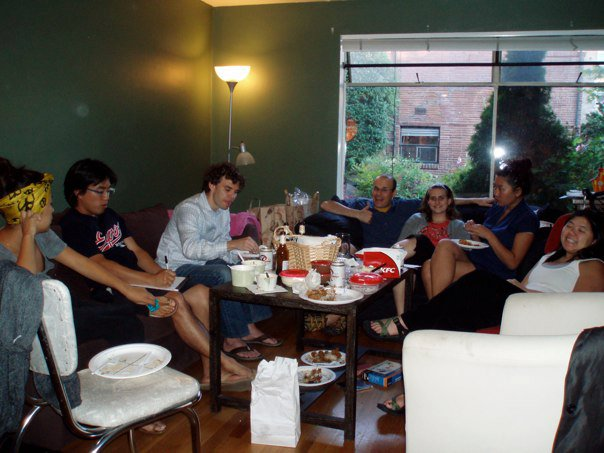
\includegraphics[height=7cm]{figure/fried_chicken}
\end{center}

\end{frame}
%------------------------------------------------------------------------------


%------------------------------------------------------------------------------
\begin{frame}
\frametitle{Next time}
Examining and visualizing numerical data
\end{frame}
%------------------------------------------------------------------------------


\end{document}










